% ------------------------------------------------------------------------------
% Este fichero es parte de la plantilla LaTeX para la realización de Proyectos
% Final de Grado, protegido bajo los términos de la licencia GFDL.
% Para más información, la licencia completa viene incluida en el
% fichero fdl-1.3.tex

% Copyright (C) 2012 SPI-FM. Universidad de Cádiz
% ------------------------------------------------------------------------------

Esta sección cubre el análisis del sistema de información a desarrollar, haciendo uso del lenguaje de modelado UML.

\section{Modelo Conceptual}
A partir de los requisitos de información, se desarrollará un diagrama conceptual de clases UML. En ella identificaremos las clases, atributos y relaciones entre ellas tal y como podemos ver en \ref{fig:digclases}.

\begin{figure}[h!]
	\begin{center} 
		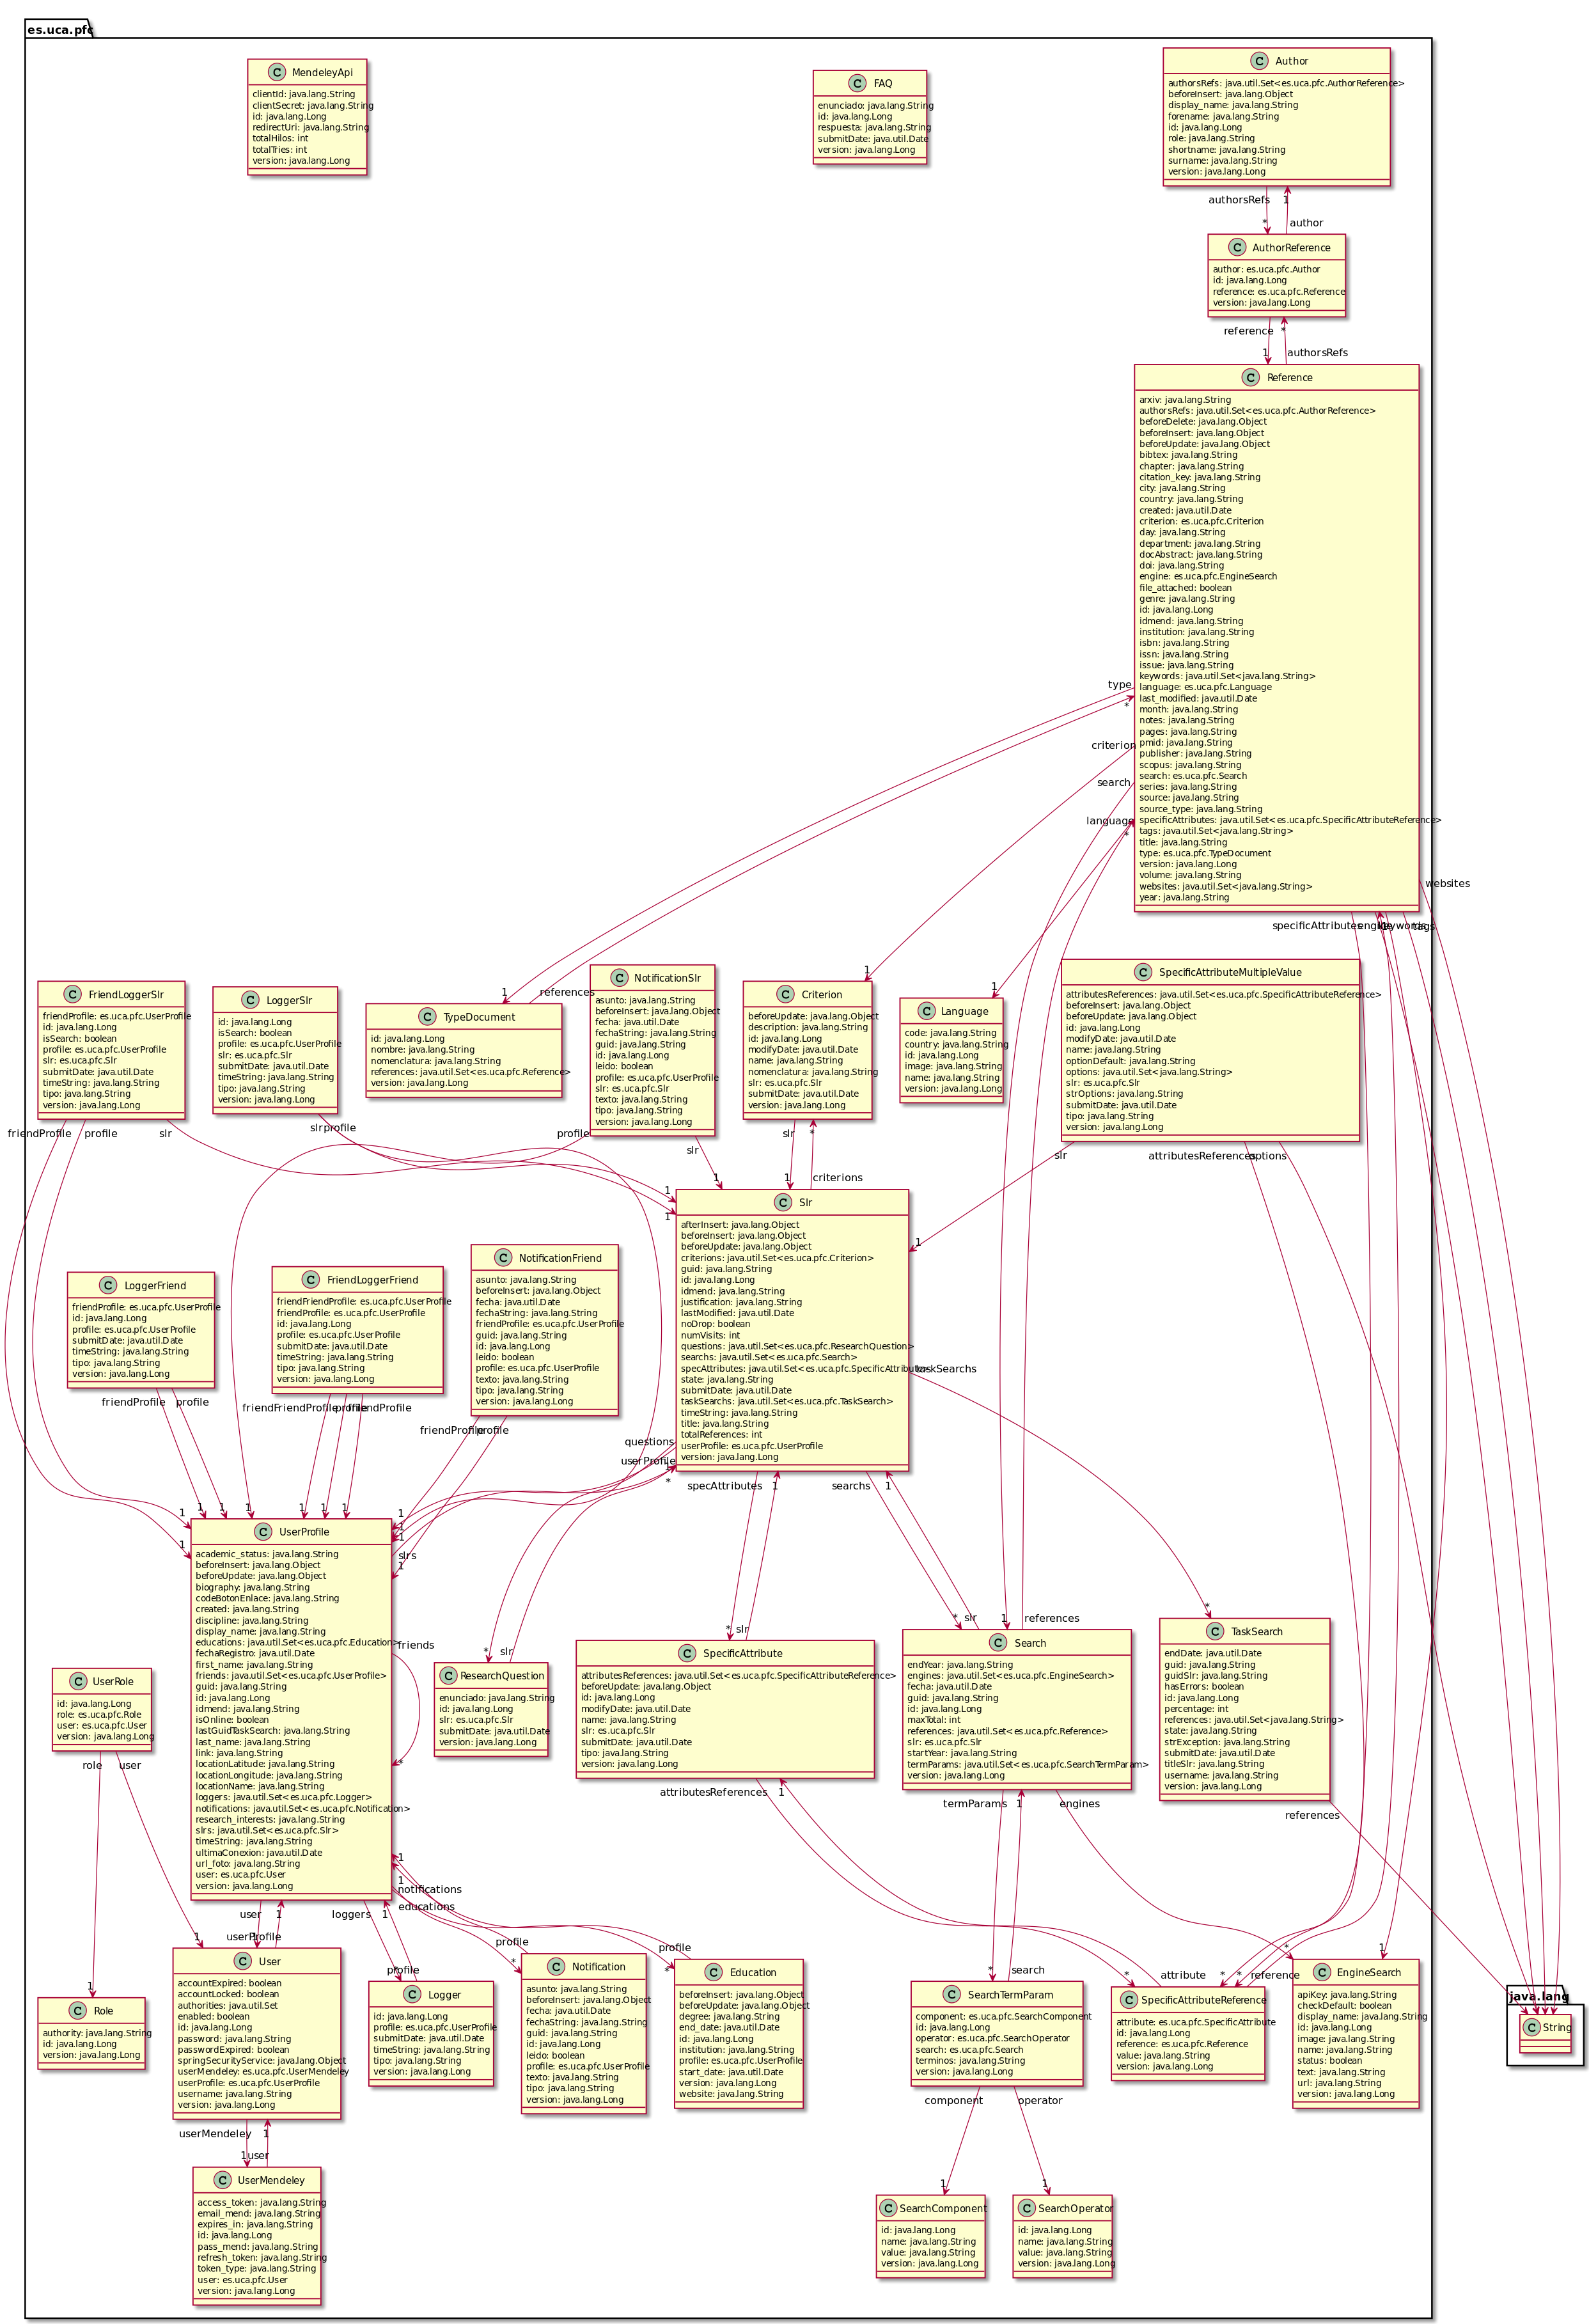
\includegraphics[width=\linewidth]{class-diagram.png}
		\caption{Diagrama conceptual de clases UML.}
		\label{fig:digclases}
	\end{center}
\end{figure}

%A partir de los requisitos de información, se desarrollará un diagrama conceptual de clases UML, identificando las clases, atributos, relaciones, restricciones adicionales y reglas de derivación necesarias.

\section{Modelo de Casos de Uso}
A partir de los requisitos funcionales descritos en apartados anteriores, se emplearan los casos de uso como mecanismo para representar las interacciones entre los actores y el sistema a desarrollar.
%A partir de los requisitos funcionales descritos anteriormente, se emplearan los casos de uso como mecanismo para representar las interacciones entre los actores y el sistema bajo estudio. Para cada caso de uso deberá indicarse los actores implicados, las precondiciones y postcondiciones, los pasos que conforman el escenario principal y el conjunto de posibles escenarios alternativos.

\subsection{Actores} 
Los diferentes roles que con el sistema pueden interactuar son los siguientes:

\begin{itemize}
	\item Investigador. Esta figura representa el usuario principal del sistema web. Una persona con este rol podrá realizar revisiones sistemáticas de la literatura y efectuar todas las tareas relacionadas con ellas.
	\item Administrador. Esta figura podrá realizar todas las funciones del rol investigador, junto con el mantenimiento de gestión de los usuarios y los errores de búsquedas de referencias bibliográficas producidas en el sistema.
\end{itemize}

%En este apartado se describirán los diferentes roles que juegan los usuarios que interactúan con el sistema. Los actores pueden ser roles de personas físicas, sistemas externos o incluso el tiempo (eventos temporales).

\subsection{Diagramas y especificación de casos de uso}
En esta sección se mostrarán los diagramas de casos de uso de la aplicación web (\ref{fig:cu01}, \ref{fig:cu02}, \ref{fig:cu03}, \ref{fig:cu04}, \ref{fig:cu05}, \ref{fig:cu06}, \ref{fig:cu07}, \ref{fig:cu08}), así como la especificación de los mismos mediante escenarios de casos de uso. Los dos primeros dígitos de la numeración de los casos de uso 

\begin{figure}[h!]
	\begin{center} 
		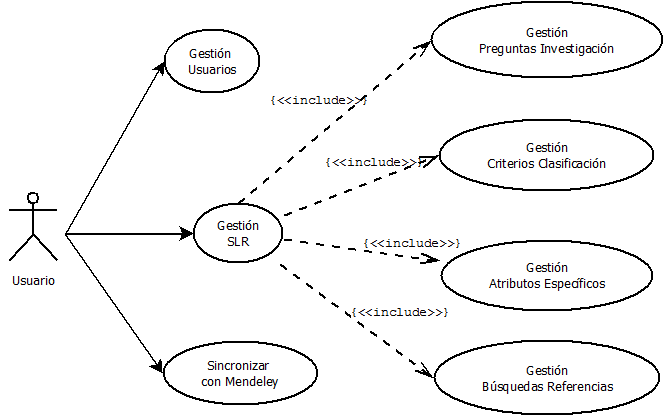
\includegraphics[scale=0.6]{cu-sistema.png}
		\caption{Diagrama casos de usos del sistema.}
		\label{fig:cu01}
	\end{center}
\end{figure}

\begin{figure}[h!]
	\begin{center} 
		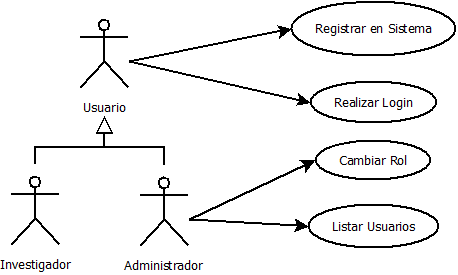
\includegraphics[scale=0.6]{cu-gestusuarios.png}
		\caption{Diagrama casos de usos de la gestión de usuarios.}
		\label{fig:cu02}
	\end{center}
\end{figure}

\begin{figure}[h!]
	\begin{center}
		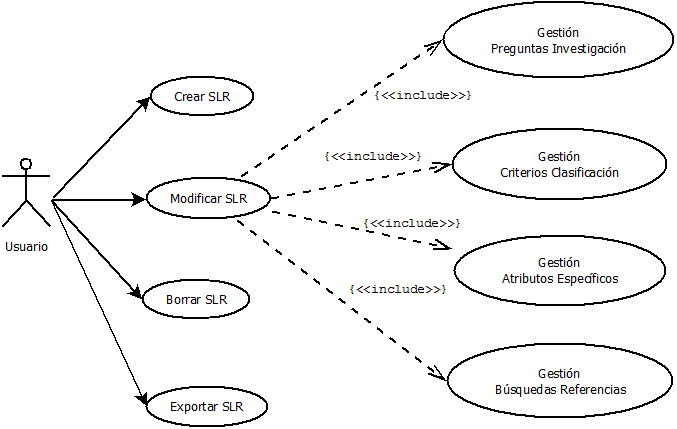
\includegraphics[scale=0.55]{cu-gestslr.png}
		\caption{Diagrama casos de usos de la gestión de revisiones sistemáticas.}
		\label{fig:cu03}
	\end{center}
\end{figure}

\begin{figure}[h!]
	\begin{center}
		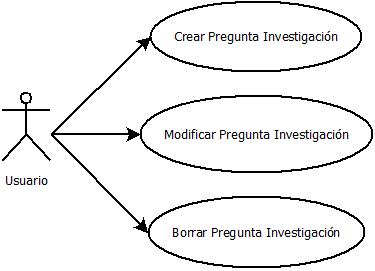
\includegraphics[scale=0.55]{cu-gestpreginv.png}
		\caption{Diagrama casos de usos de la gestión de preguntas de investigación.}
		\label{fig:cu04}
	\end{center}
\end{figure}

\begin{figure}[h!]
	\begin{center}
		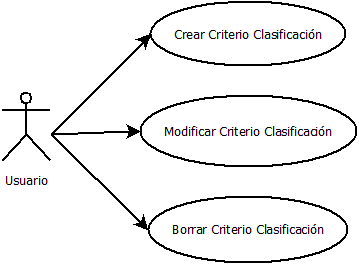
\includegraphics[scale=0.55]{cu-gestcrit.png}
		\caption{Diagrama casos de usos de la gestión de criterios de clasificación.}
		\label{fig:cu05}
	\end{center}
\end{figure}

\begin{figure}[h!]
	\begin{center}
		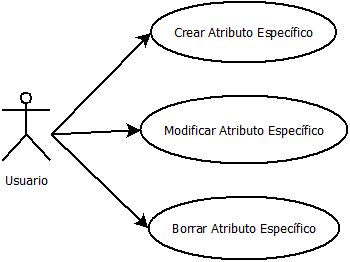
\includegraphics[scale=0.55]{cu-gestatesp.png}
		\caption{Diagrama casos de usos de la gestión de atributos específicos.}
		\label{fig:cu06}
	\end{center}
\end{figure}

\begin{figure}[h!]
	\begin{center}
		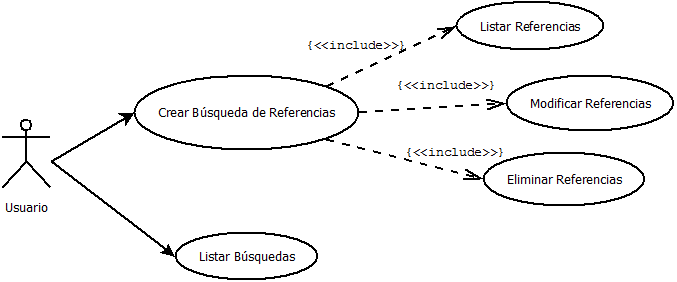
\includegraphics[scale=0.55]{cu-gestbusquedas.png}
		\caption{Diagrama casos de usos de la gestión de búsquedas de referencias bibliográficas.}
		\label{fig:cu07}
	\end{center}
\end{figure}

\begin{figure}[h!]
	\begin{center}
		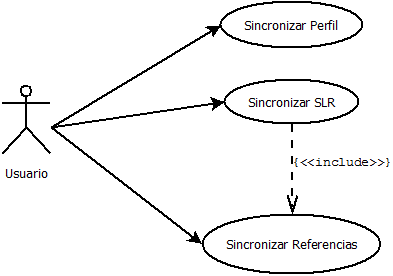
\includegraphics[scale=0.55]{cu-sincromend.png}
		\caption{Diagrama casos de usos de la sincronización con Mendeley.}
		\label{fig:cu08}
	\end{center}
\end{figure}


\section{Modelo de Comportamiento}
A partir de los casos de uso anteriores, se crea el modelo de comportamiento. Para ello, se realizarán los diagramas de secuencia del sistema, donde se identificarán las operaciones o servicios del sistema. Luego, se detallará el contrato de las operaciones identificadas.

\section{Modelo de Interfaz de Usuario}
En esta sección se deberá incluir un prototipo de baja fidelidad o mockup de la interfaz de usuario del sistema. Además, es preciso elaborar un diagrama de navegación, reflejando la secuencia de pantallas a las que tienen acceso los diferentes roles de usuario y la conexión entre éstas.